\documentclass[12pt, spanish]{article}
\usepackage[spanish]{babel}
\selectlanguage{spanish}
\usepackage{natbib}
\usepackage{url}
\usepackage[utf8x]{inputenc}
\usepackage{graphicx}
\graphicspath{{images/}}
\usepackage{parskip}
\usepackage{fancyhdr}
\usepackage{vmargin}

\usepackage[default]{sourcesanspro}

\setmarginsrb{2 cm}{1 cm}{2 cm}{2 cm}{1 cm}{1.5 cm}{1 cm}{1.5 cm}

\title{Sistemas Operativos:\\
Trabajo Tema 1  \hspace{0.05cm} }   

\author{Pedro Jiménez Alférez \\
Marina Hernádez Bautista  \\
Juan Carlos González Quesada \\
Román Larrosa Lewandowska \\
María Sánchez Marcos \\
Antonio David Villegas Yeguas	}                             

\renewcommand*\contentsname{hola}

\makeatletter
\let\thetitle\@title
\let\theauthor\@author
\let\thedate\@date
\makeatother

\pagestyle{fancy}
\fancyhf{}
\rhead{}
\chead{\thedate}
\lhead{\thetitle}
\cfoot{\thepage}

\begin{document}
%%%%%%%%%%%%%%%%%%%%%%%%%%%%%%%%%%%%%%%%%%%%%%%%%%%%%%%%%%%%%%%%%%%%%%%%%%%%%%%%%%%%%%%%%

\begin{titlepage}
    \centering
    \vspace*{0.5 cm}
    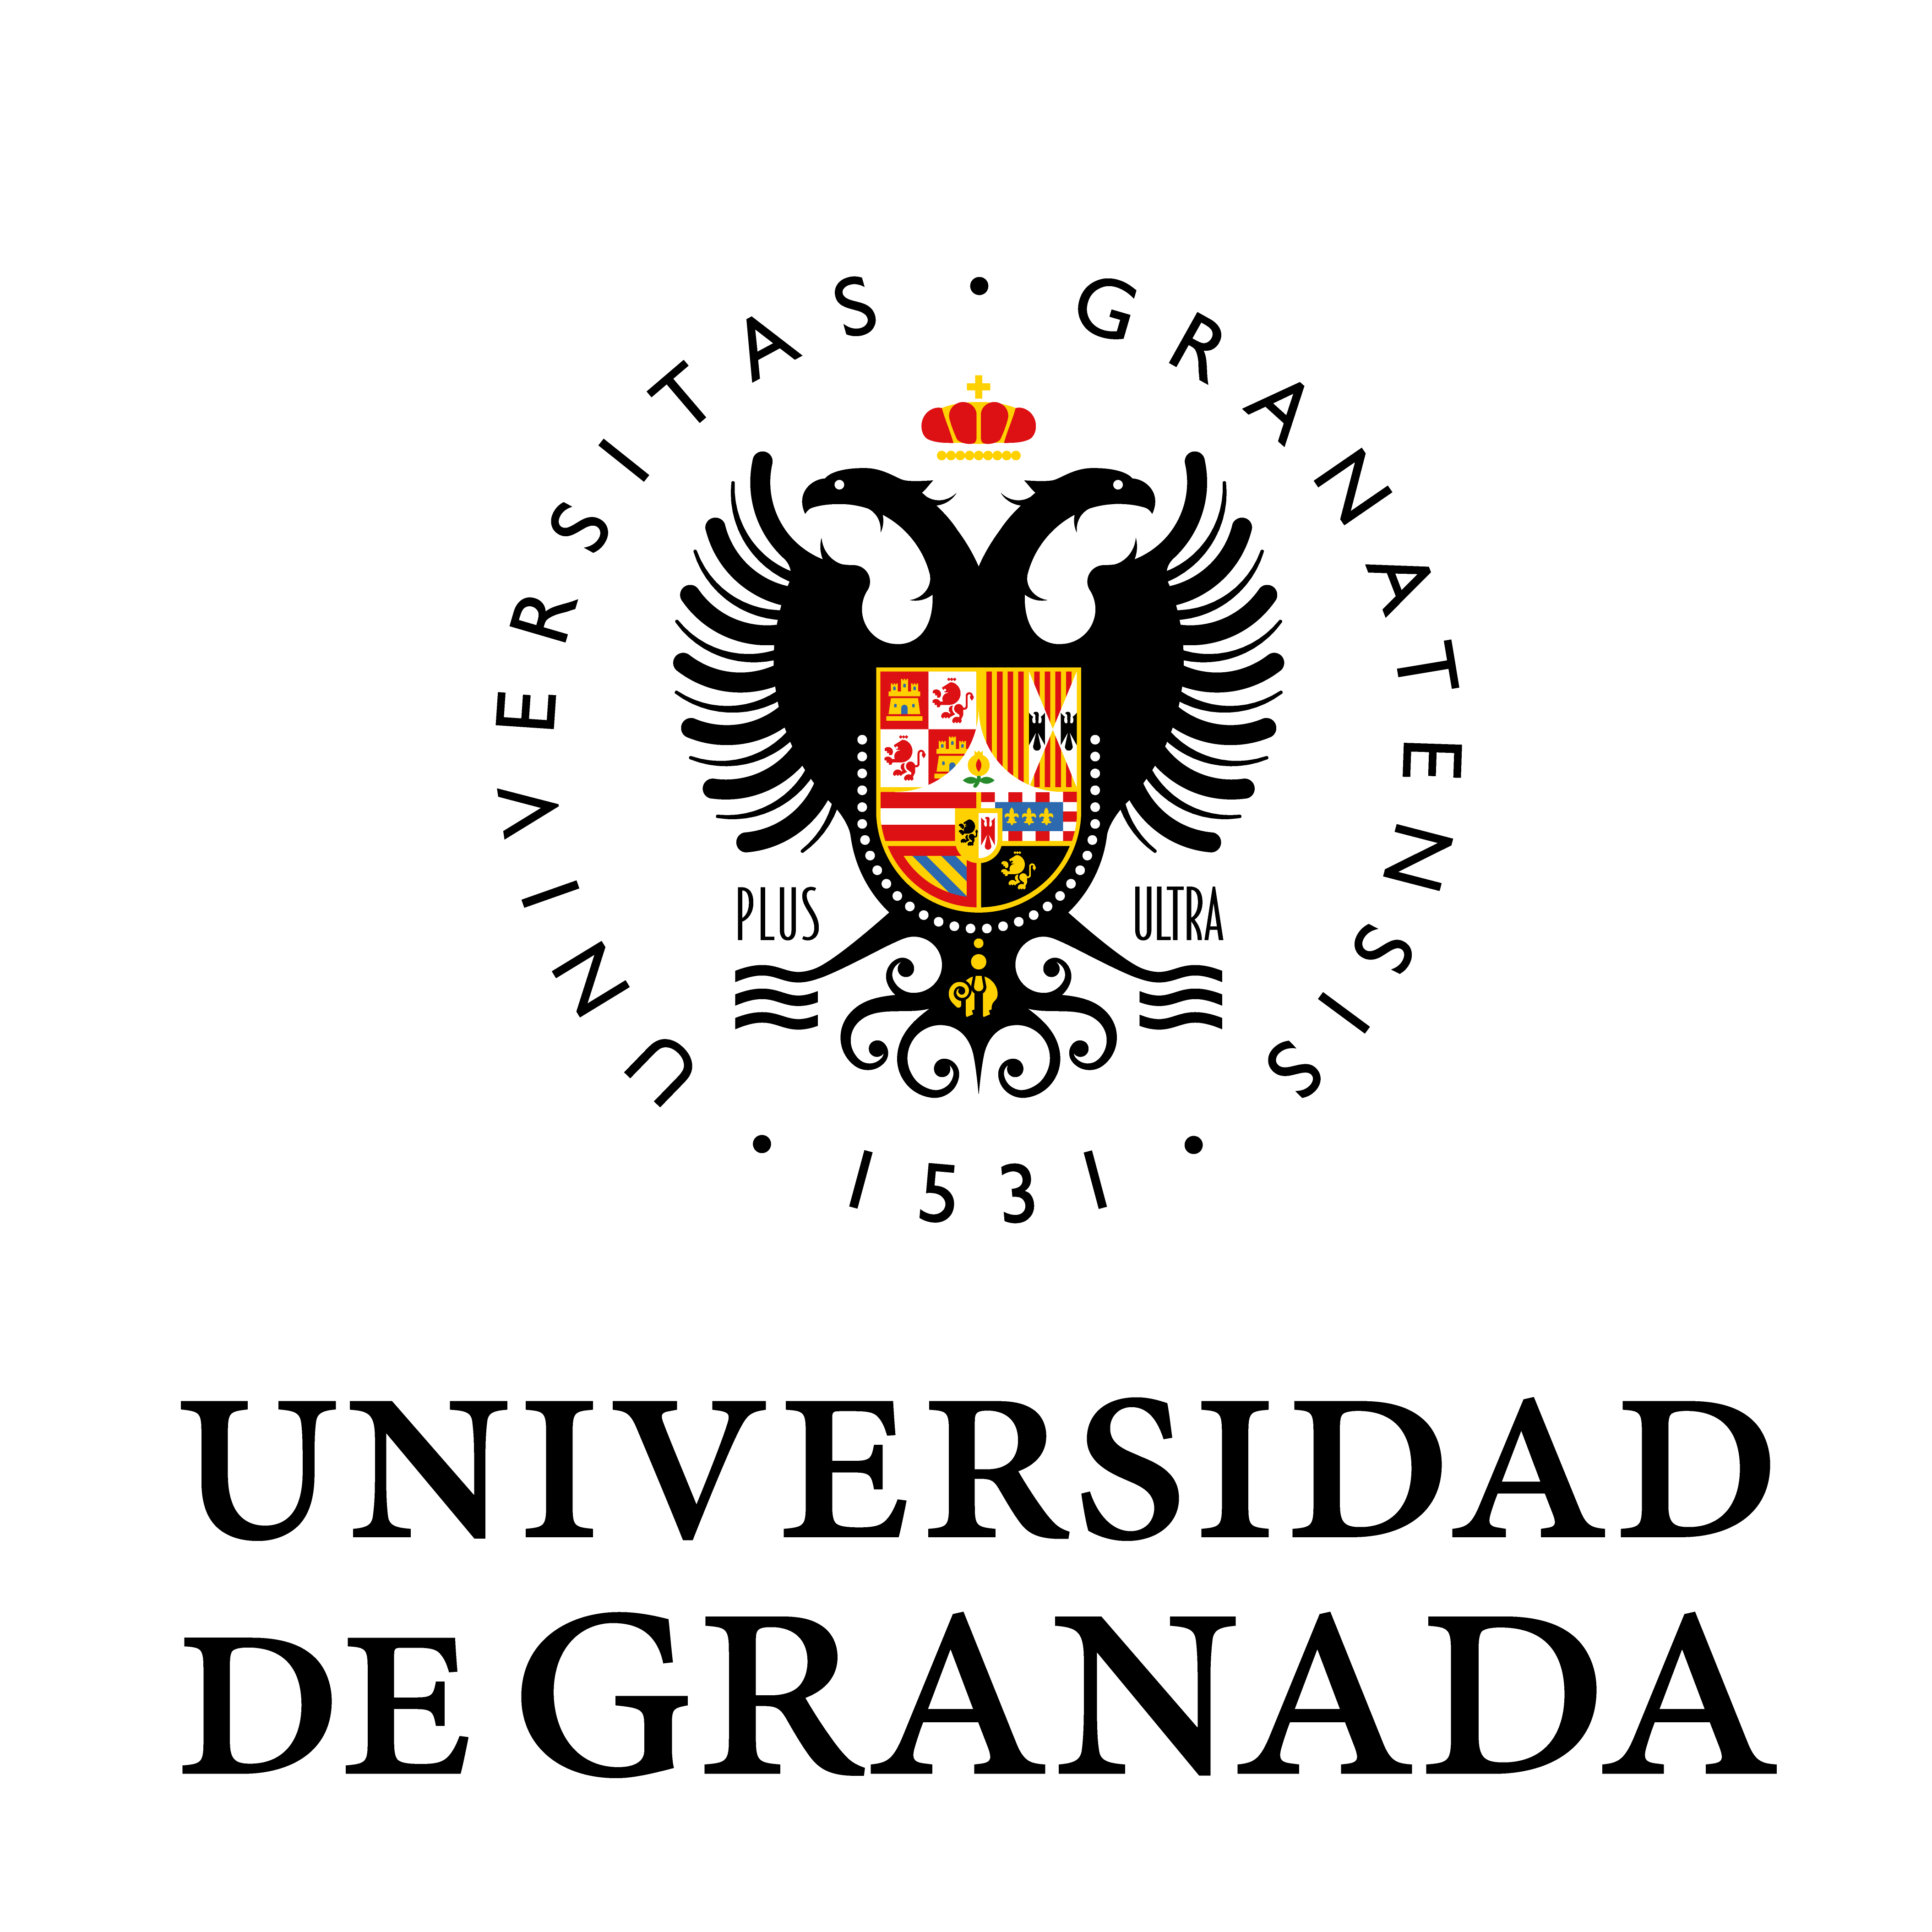
\includegraphics[scale = 0.50]{ugr.png}\\[1.0 cm]
    %\textsc{\LARGE Universidad de Granada}\\[2.0 cm]   
    \textsc{\large 2ºB}\\[0.5 cm]            
    \textsc{\large Grado en Ingeniería Informática}\\[0.5 cm]              
    \rule{\linewidth}{0.2 mm} \\[0.4 cm]
    { \huge \bfseries \thetitle}\\
    \rule{\linewidth}{0.2 mm} \\[1.5 cm]
    
    \begin{minipage}{0.4\textwidth}
        \begin{flushleft} \large
            \emph{Autores:}\\
            
            \small \theauthor
            \end{flushleft}
            \end{minipage}~
            \begin{minipage}{0.4\textwidth}
            \begin{flushright} \large
            \emph{Asignatura: \\
            Sistemas Operativos}                   
        \end{flushright}
    \end{minipage}\\[1 cm]
  	
    {\small \thedate}\\[1 cm]
 	
    \vfill
    
\end{titlepage}

\newpage

%%%%%%%%%%%%%%%%%%%%%%%%%%%%%%%%%%%%%%%%%%%%%%%%%%%%%%%%%%%%%%%%%%%%%%%%%%%%%%%%%%%%%%%%%


\tableofcontents
\pagebreak

%%%%%%%%%%%%%%%%%%%%%%%%%%%%%%%%%%%%%%%%%%%%%%%%%%%%%%%%%%%%%%%%%%%%%%%%%%%%%%%%%%%%%%%%%

\section{Introducción}

La elección de este sistema operativo se debe a que Arch Linux es una distribución poco conocida. Además, como uno de los miembros de nuestro grupo lo utiliza, tenemos más experiencia sobre su funcionamiento, a la vez que el resto de miembros del grupo ampliamos nuestro conocimiento relativo a otras distribuciones de GNU/Linux.

Como la mayoría de distribuciones GNU/Linux, Arch Linux está formado por software libre, permitiendo a los usuarios acceder al código, modificarlo y actualizarlo. La licencia que utiliza el kernel de distribución es GNU GPLv2.Se trata de una distribución GNU/Linux de propósito general cuyo funcionamiento se basa en el principio de diseño KISS (“Keep It Simple, Stupid!”). Es un SO que intenta mantener un entorno sencillo y minimalista para permitir a los usuarios la modificación de su contenido y propiedades.


A partir del 25 de enero 2017 el soporte para arquitecturas i686 (procesadores de 32 bits) fue descontinuado, aunque se sigue manteniendo la paquetería de 32 bits disponible para las arquitecturas x86-64, los equipos que utilizan procesadores de 32 bits no pueden usar esta distribución (de forma oficial, y mantenida por los desarrolladores de la distribución). Aunque pueda parecer que esto deja a muchos usuarios sin soporte, hay que puntualizar que incluso una de las distribuciones más usadas de GNU/Linux (Ubuntu) los usuarios que la tienen instalada en un procesador de 32 bits es menor al 2\% por lo que esto no tiene por que suponer un problema.


\section{Historia}

La distribución Arch Linux es una de las más influyentes a nivel comunitario, sin embargo esto no siempre fue así. Los desarrolladores de la distribución son voluntarios no remunerados, y no hay perspectivas de monetizar la distribución, por lo que seguirá siendo de libre uso.

Arch Linux 0.1 fue lanzado el 11 de marzo de 2002, un año después de que su creador, Judd Vinet, comenzase a desarrollarlo motivado por crear una distribución de GNU/Linux sencilla como las ya existentes en el momento Slackware, CRUX, entre otras. Otra de las motivaciones de su creador fue la falta de gestores de paquetes, por lo que también creó un programa de gestión de paquetes, Pacman, que aún hoy es el usado en la distribución.

La comunidad de Arch Linux fue creciendo, y desde sus primeros días se alzó como una comunidad muy colaboradora y unida por el fin mismo de la distribución: Mantener la simplicidad y servir de utilidad a sus usuarios, en lugar de querer acaparar la mayoría de usuarios.

\newpage

\section{Gestor de paquetes}

\subsection{Oficial: Pacman}

Pacman es el gestor de paquetes por defecto de Arch Linux. Este gestor está programado en lenguaje C y usa el formato tar para la compresión de paquetes.

La característica principal de Pacman es que permite administrar tanto archivos de repositorios del SO como archivos que han sido creados por el usuario. 

Como esta distribución es tipo rolling release, sus actualizaciones son frecuentes y pequeñas, a diferencia del estándar normal, que actualiza y reinstala las actualizaciones sobre la versión anterior. El gestor de archivos permite instalar y actualizar paquetes mediante comandos del programa.

\subsection{Comunitarios}

Ademas, existen gestores de paquetes creados por la comunidad, capaces de instalar los programas creados y mantenidos por la comunidad, en un repositorio externo al oficial, pero aun así, en los servidores de la distribución (Arch User Repository)

\newpage

\section{Arquitectura de ficheros}

Como la mayoría de Sistemas Operativos que usan el núcleo de Linux como hemos visto en prácticas, Arch Linux utiliza el sistema FHS (Filesystem Hierarchy Standard). El FHS es un estándar que propone una forma sistemática de organizar toda la información que almacena un sistema operativo tipo Linux. Esta arquitectura se basa en una gestión de directorios en forma de árbol, donde la raíz del sistema se representa en el directorio $"$ / $"$, y a partir de este, cuelgan los demás.

Este estándar es el propuesto por The Linux Fundation.

\subsection{Esquema FHS}
El estándar FHS sigue los siguientes directorios y almacena la siguiente información:

\begin{itemize}
	\item{\textbf{/bin} : Programas de utilidad fundamentales para ser utilizados por cualquier usuario}
	\item{\textbf{/sbin} : Programas de utilidad fundamentales para ser utilizados por el usuario root.}
	\item{\textbf{/boot} : Archivos fundamentales para el programa Boot Loader.}
	\item{\textbf{/dev} : Todos los archivos especiales de dispositivo.}
	\item{\textbf{/etc} : Archivos de configuración del sistema.}
	\item{\textbf{/home} : Los directorios de inicia de todos los usuarios que disfrutan de una cuenta en el sistema, excepto, el directorio de inicio del root: /root}
	\item{\textbf{/lib} : Bibliotecas sin las que no pueden funcionar los programas ubicados en /bin y /sbin.}
	\item{\textbf{/media} : Este directorio actúa como punto de montaje para dispositivos extraibles: DVD-ROM, dispositivos USB, etc.}
	\item{\textbf{/mnt} : Este directorio actúa como punto de montaje para sistemas de archivos montados temporalmente.}
	\item{\textbf{/opt} : Normalmente aquí se ubican los programas que no forman parte de la distribución instalada en el sistema.}
	\item{\textbf{/proc} : Sistema de archivos virtual que hace de interfaz con el núcleo y los procesos.}
	\item{\textbf{/tmp} : Archivos temporales que normalmente no se mantienen una vez se apaga el sistema.}
	\item{\textbf{/usr} : Archivos ejecutables, archivos de código fuente, bibliotecas, documentación y, en general, todos los programas y utilidades.}
	\item{\textbf{/var} : Los archivos cuyo contenido se espera que cambie durante el funcionamiento normal del sistema.}
\end{itemize}



\section{Núcleo}

Arch Linux usa el kernel (núcleo) Linux, de tipo monolítico.

Un kernel de tipo monolítico, implica que el kernel es un único ejecutable (como hemos visto en prácticas, el archivo  vmlinu*), en el que el sistema depende de un procedimiento principal (como hemos visto en clase, el proceso con PID 0) y a partir de ese proceso, se genera una estructura de procesos en forma de árbol.


Este kernel sigue una estructura modular, permitiendo la gestión del sistema en forma de módulos, que se podrán cargar en el núcleo mientras están en memoria (enlace dinámico), o gestionar los módulos de forma jerárquica(módulos apilables), los módulos sirven como bibliotecas


\vspace{5cm}


\bibliographystyle{plain}
\bibliography{biblist}


\end{document}